\RequirePackage[hyphens]{url}

\documentclass[sigconf]{acmart}

\usepackage{graphicx}
\usepackage{hyperref}
\usepackage{todonotes}

\usepackage{endfloat}
\renewcommand{\efloatseparator}{\mbox{}} % no new page between figures

\usepackage{booktabs} % For formal tables

\settopmatter{printacmref=false} % Removes citation information below abstract
\renewcommand\footnotetextcopyrightpermission[1]{} % removes footnote with conference information in first column
\pagestyle{plain} % removes running headers

\newcommand{\TODO}[1]{\todo[inline]{#1}}

\usepackage{listings}
\usepackage{color}
% \usepackage[parfill]{parskip}

\definecolor{dkgreen}{rgb}{0,0.6,0}
\definecolor{gray}{rgb}{0.5,0.5,0.5}
\definecolor{mauve}{rgb}{0.58,0,0.82}

\lstset{frame=tb,
  language=Python,
  aboveskip=3mm,
  belowskip=3mm,
  showstringspaces=false,
  columns=flexible,
  basicstyle={\small\ttfamily},
  numbers=none,
  numberstyle=\tiny\color{gray},
  keywordstyle=\color{blue},
  commentstyle=\color{dkgreen},
  stringstyle=\color{mauve},
  breaklines=true, 
  breakatwhitespace=true
  tabsize=3
}

\def\bZ{\mathbb{Z}}
\def\bN{\mathbb{N}}
\def\bR{\mathbb{R}}
\def\bC{\mathbb{C}}
\def\bQ{\mathbb{Q}}

\usepackage{indentfirst}
 
\begin{document}
\title{Diagnosis of Coronary Artery Disease Using Big Data Analysis}


\author{Hady Sylla}
\affiliation{%
  \institution{Indiana University Bloomington}
  \city{Bloomington} 
  \state{Indiana} 
  \postcode{47401}
}
\email{hsylla@iu.edu}



% The default list of authors is too long for headers}
\renewcommand{\shortauthors}{H. Sylla}


    
\begin{abstract}
Coronary disease is the most common heart disease. Coronary disease is the primary cause of heart attack and death in the world \cite{ali}. Early diagnostic of this illness is, therefore, of great importance. Some techniques have up to this point been conceived for diagnosing coronary. In spite of the significant change in future in recent years, there are difficulties that are putting weight on the managed capacity healthcare system. This exceptional circumstance is offering the right energy to reconsider plans of action on healthcare services frameworks which require another vital approach moving from a volume to an execution based model-value for money \cite{ali}.
Presently big data does not productively contribute to enhancing healthcare. In an inexorably engaged computerized society, enormous information has now achieved each area in the worldwide economy. Individual information has turned into another type of currency, in any case, this "cash" isn't owing in the therapeutic services division since patients are not in control of their medical health data making impossible to build the trust that is needed.
\end{abstract}


\keywords{i523, hid339, Coronary disease, big data, Random Forest}


    \maketitle
    
\subsection{Introduction}

The Coronary artery disease (CAD) comes about when atherosclerotic plaques develops in the coronary arteries giving rise to the narrowing of coronary luminal, and sometimes, occlusion, which leads to heart failure or a sudden cardiac failure. In western nations, CAD is among the killer  diseases. It is important for people understand the CAD”s pathophysiology, how to control its development, identifying and effective innovation of the cardiovascular risk elements, and how to diagnose and treat it in early stages, and its reversible stages. The experts consider big data mining technique as “gold standard” for diagnosing CAD and it is common in use. However, big data mining is an expensive and invasion procedure that requires a high-level of technological experience and latest technology thus the medical experts cannot use it to screen many patients or treat them.  Due to this, many health facilities utilizes other noninvasive tools to diagnose CAD. The most popular of these methods are stress echocardiography (ECHO), electrocardiogram (ECG), and scintigraphy or SPECT. Additionally, the clinical set ups currently use the coronary magnetic resonance angiography (CMRA) MSCT or EBCT. The objective of this study is showing how using big data mining technique to diagnose the Coronary Artery Disease is the best way to control heart attacks and deaths. The study discusses the features in the big data mining tool, how they derive the results, and discussion of the results. Additionally, the research gives way to future studies and offers recommendations to improve the CAD complication field. 
Data mining is a technique of finding hidden information in a database. Nowadays, several fields use data mining as it has different applications like scientific discoveries, in entrepreneurship, and fraud detention. Data mining calculations work on databases, in which each information archive has several attributes.  One of these attributes is the class label, which discovers the data category. The data mining algorithms people use in problems solving are association rule mining, classification, regression analysis and clustering.
To classify algorithms, a researcher requires a learning phase on a labeled data set, which makes him/her make a decision on the missing test record class label. In the learning phase, a scientist constructs a classification model to predict the data label class label using its values features. Specialist categorizes heart complications as cardiovascular and cardiomyopathy disorders. The Coronary Artery Disease (CAD) is a major cardiomyopathy complication subgroup which causes disability, serious illness, and even death as the disease affect oxygen and blood supply to the heart muscles. The early symptoms of heart disease comprise pain in the center of the chest or a sense of numbness, and palpitation. Other signs are fainting fits or dizzy spells, and dyspnea on exertion. 
Due to the grave nature of heart failures, it is important to find out its causes. Currently, the major goal of many scientific pursues is making accurate diagnosis of cardiac complications. The researchers collect a great deal of information while examining CAD patients, and by processing the information they reveal how the main features of cardiac disorders relate (e.g. the amount of cholesterol, blood pressure, etc.) and these complications’ occurrence probability. The next chapter discusses several research articles that discuss this topic and relate it to what this study’s findings.


\section{Background}

 The study by  \cite{ali} daiagnoses of coronary altery disease using HRV features and applies several algorithms like SVM, CPAR, C 4.5 and CMAR to them by expressing the performance in terms of Recall, TP, Precision, and TP \citep{ali}. From the study by Lee et al., the SVM algorithm exhibits an excellent performance. Another research by Srivinivas et al. (2010) archives an accuracy of eighty-four percent by probing into why the clogging of the main heart vessels i.e. the right coronary artery, the left circumflex artery, and the left anterior descending coronary artery.	Kavitha and Ramakrishnan (2010) use the genetic and neutral algorithms to diagnose CAD and were successful in ensuring the technique works. In another study, Wang and Hoy (2005) employ features like blood pressure, sex, smoking, age, high-density lipoprotein cholesterol (HDL), and cholesterol to diagnose CAD. Wang and Hoy (2005) also uses the Framingham function to perform the CAD diagnosis.  Another study by Palaniappan and Awang (2008) draws upon a limited count of the features the paper mentions above regarding three different data mining algorithms, which are the Naïve Bayes, neural network, and decision. The results from their research show an accuracy rate of 85.53 percent. Shantakumar and Kumaraswamy (2009) use thirteen features and neural network algorithm to design a system which predicts heart attack.	Apparently, for all studies reviewers conduct regarding this field, the work of some physical examination and the ECG features in the diagnosis of CAD is not clear.  To address this issue in the current literature, the latest studies investigate the effect of a wide set of physical examination and ECG features while diagnosing CAD. These modern features the analysis includes are the Q wave, dyspnea, T inversion, New York Heart Association’s functional class,  ST elevation, and the ST depression. So far, the scientists have not conducted studies regarding these features’s context. Amongst the entire data mining associations rule, algorithms, and classifications is where the researchers select the mining techniques basing on the aim of the study. The study constructs a dataset from the information it gets from three hundred and three impromptu visitors (two hundred and sixteen patients) to Shaheed Rajaei Cardiovascukar, Medical and Research Center. Then the research uses the dataset to analyze the impacts of different ECG , demographic, and clinical features while diagnosing  CAD. The study utilizes different classification algorithms to evaluate the dataset; these include proposed ensemble, Naïve Bayes, and SMO algorithm. Furthermore, it employs ten-fold cross-validation to assess the accuracy of the evaluations. The research uses the findings of the standard angiographic tool as a basis for comparison to assess the ability to predict the classification algorithms. Below are the aims of the study:
I.	The analysis of the technique to predict CAD and prevent highly troublesome and invasive procedures like angiography;
II.	Detection of the features efficiency in the CAD diagnosis;
III.Anticipation of the CAD incidence by using data mining tools;
IV.	Innovation of a database on CAD, comprising effective elements and their weights;
V.	Finding efficient analytical techniques to evaluate the collected dataset; and
VI.	Analyzing the tool for CAD diagnosis by test and training sets.
The other part of the research paper’s organization is as follows: Section 3 evaluates the dataset, Section 4 does the introduction of algorithms, and section 6 gives the conclusions and recommendations for future research regarding the topic.

\section{Dataset}
For this project I will use Z-Alizadeh Sani aataset for the data analuysis.
The dataset elements comprise of ECG features, demographics, and symptoms and physical examinations. 
The class attribute is Cath which the angiography determines. If the diameter narrowing is bigger than or equivalent to fifty percent, the class value is CAD, Normal otherwise. In the features the study analyses above, “DM” means the history of diabetes mellitus, “HTN” is the history of hypertension, and “Ex-smoker” refers to candidates with a past smoking character. Additionally, “FH” is an individual’s heart disease history in the first-degree relatives, and “Current Smoker” means someone who smokes. Moreover, the study uses the discretizationranges it offers in the Braunwald’s Heart Disease book for enriching the dataset.

\subsection{Methodology}

The study employs three classification algorithms to evaluate the dataset. In this part, the paper describes the data mining algorithms I uses to analyze the dataset.

\section{Risk factors}
\par In spite of the fact that an extensive variety of hazard factors for coronary heart dis-ease have been distinguished from populace ponders, these measures, separately or in blend, are inadequately pow-erful to give a solid, noninvasive conclusion of the nearness of coronary illness. Here we demonstrate that pat-tern-acknowledgment systems connected to proton atomic mag-netic reverberation (1H-NMR) spectra of human serum can effectively analyze the nearness, as well as the seriousness, of coronary illness. Utilization of super-vised halfway minimum squares-discriminant examination to orthogo-nal flag amended informational collections permits >90\% of subjects with stenosis of every one of the three noteworthy coronary vessels to be distin-guished from subjects with angiographically ordinary coro-nary supply routes, with a specificity of >90\%. Our examinations appear out of the blue a system fit for giving an accu-rate, noninvasive and fast conclusion of coronary heart dis-facilitate that can be utilized clinically, either in populace screening or to permit compelling focusing of medicines, for example, statins.
Coronary illness (CHD) is a noteworthy reason for mortality and bleakness in created nations, influencing upwards of one of every three people previously the age of 70 years1. In the course of recent decades a scope of ecological and biochemi-cal chance elements for the advancement of CHD have been iden-tified in cross-sectional studies2. For instance, tobacco smoking is related with a roughly two-overlap in-wrinkled danger of CHD3. Additionally, abnormal amounts of cholesterol in substantial, triglyceride-rich lipoprotein particles (mostly low-thickness lipoprotein (VLDL) and low-thickness lipoprotein (LDL)) and lower levels of cholesterol in high-thickness lipoprotein (HDL) particles are known to be related with expanded danger of CHD4.
As of late, be that as it may, there have been specialized advances that have permitted to a great degree high-thickness informational collections to be developed from people. Methods, for example, genomics, proteomics and metabonomics (a frameworks way to deal with ex-amining the adjustments in hundreds or thousands of low-mol-ecular-weight metabolites in an in place tissue or biofluid9) offer the possibility of effectively recognizing people with specific malady or lethal states. Of these methods, NMR-based metabonomics offers a few particular preferences in a clinical setting. To begin with, it can be completed on standard arrangements of serum, plasma or urine10,11, evading the requirement for master arrangements of cell RNA and ace tein required for genomics and proteomics, respectively12– 14. Second, huge numbers of the hazard factors effectively recognized, (for example, levels of different lipids) are little atom metabolites that will add to the metabonomic informational collection.

\section{Analytic}
I will use Random Forest machine learning for predicting the feature to diagnose coronary artery disease.

Machine learning is branch of Data Science which consolidates a huge arrangement of measurable strategies. These methods enable data scientists to make a model which can gain from past information and distinguish designs from huge, uproarious and complex informational indexes. Scientists utilize machine learning for disease expectation and guess. Machine learning permits inductions or choices that generally can't be made utilizing regular measurable systems. With a powerfully approved machine learning model, odds of right finding move forward. It uncommonly helps in understanding of results for marginal cases

Machine learning utilizes features (i.e. factors or properties) to create predictive models. Utilizing an appropriate mix of highlights is fundamental for acquiring high exactness and precision. Since too much (unspecific) features pose the problem of overfitting the model, we generally want to restrict the features in our models to those, that are most relevant for the response variable we want to predict. Using as few features as possible will also reduce the complexity of our models, which means it needs less time and computer power to run and is easier to understand.

\subsection{Package Installation}

I installed the following packages in the Python environment, and load the data using panda Dataframe. Data exploration, manipulation, and visualization start with loading data, be it from files or from a URL. Pandas has become the go-to library for all things data analysis in Python.

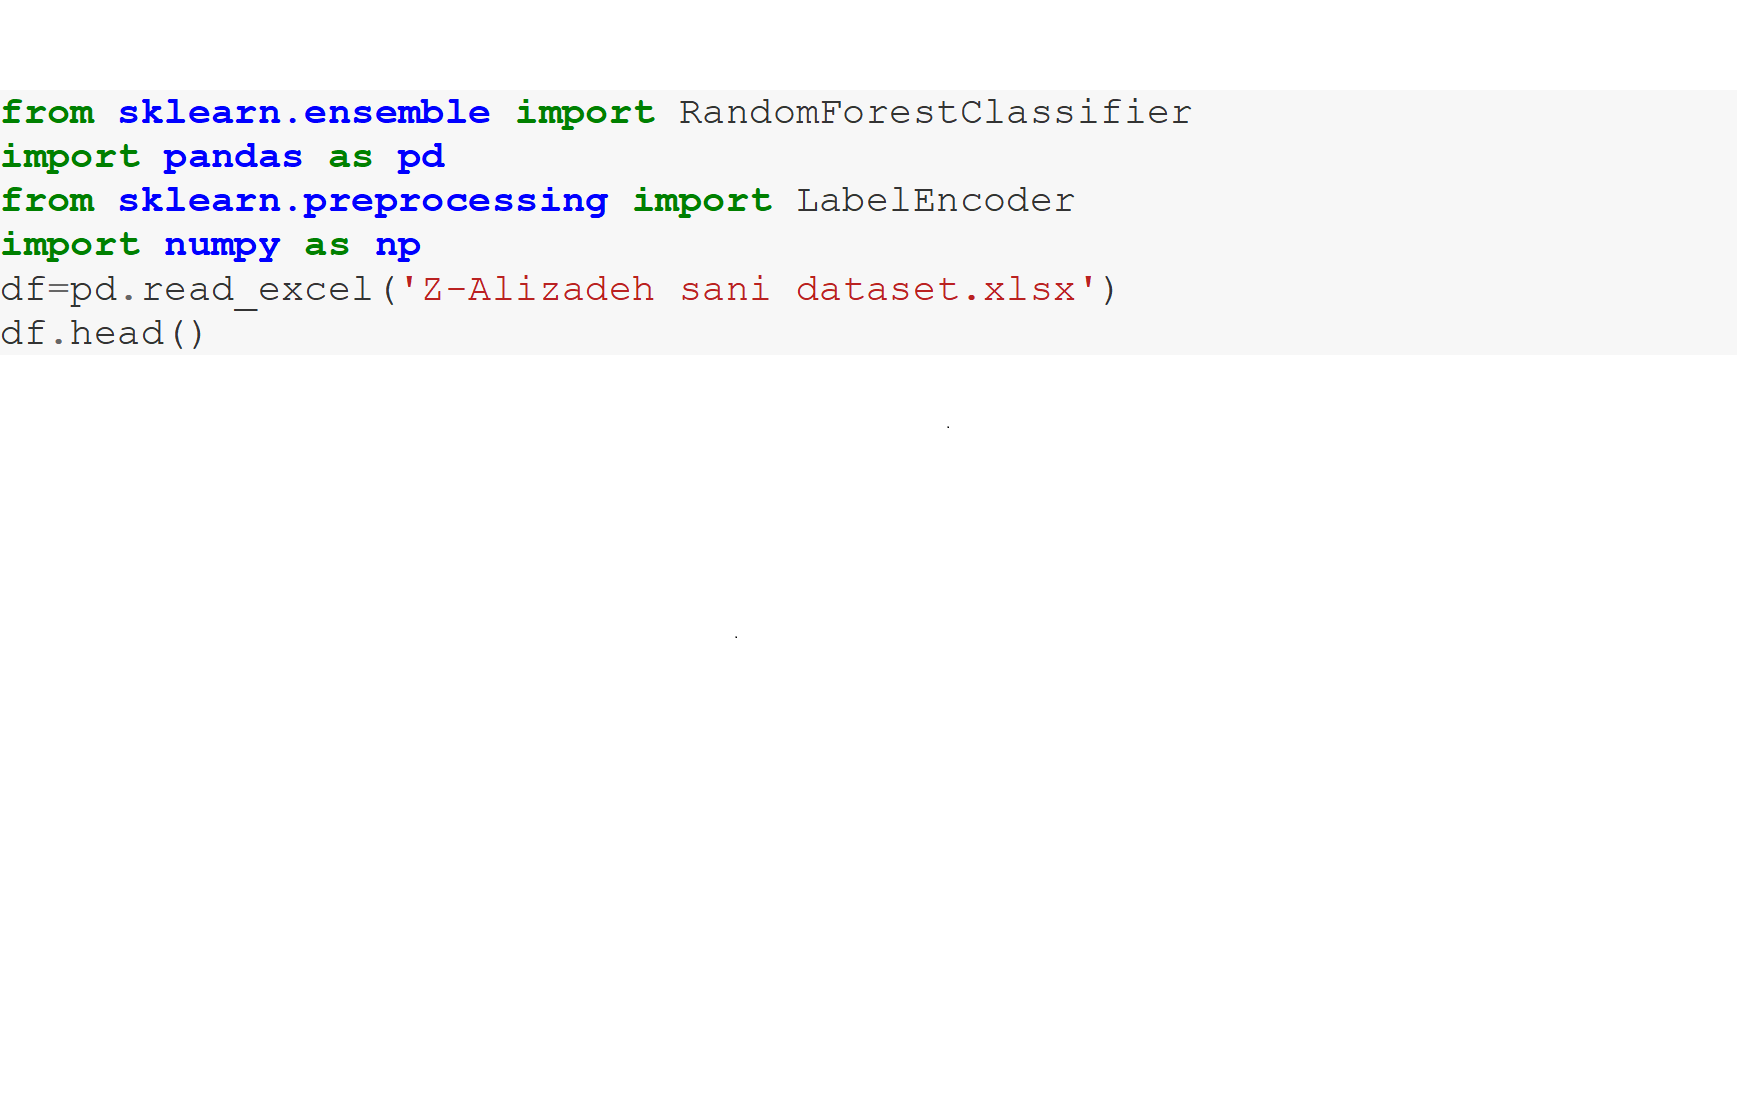
\includegraphics[width=0.95\columnwidth]{images/Untitled1.png}

I am using the describe() method that will give me basic statistics for every column in the dataset. This method will allow me to Generates descriptive statistics that summarize the central tendency, dispersion and shape of a dataset.
df.head()

\begin{table}[]
\centering
\caption{Dastaset Description}
\label{my-label}
\begin{tabular}{llllllllllllllllllllll}
Age & Weight & Length & Sex & BMI   & DM        & HTN & Current Smoker & EX-Smoker & FH & ... & K   & Na  & WBC & Lymph & Neut & PLT & EF-TTE & Region RWMA & VHD & Cath   &        \\
0   & 53     & 90     & 175 & Male  & 29.387755 & 0   & 1              & 1         & 0  & 0   & ... & 4.7 & 141 & 5700  & 39   & 52  & 261    & 50          & 0   & N      & Cad    \\
1   & 67     & 70     & 157 & Fmale & 28.398718 & 0   & 1              & 0         & 0  & 0   & ... & 4.7 & 156 & 7700  & 38   & 55  & 165    & 40          & 4   & N      & Cad    \\
2   & 54     & 54     & 164 & Male  & 20.077335 & 0   & 0              & 1         & 0  & 0   & ... & 4.7 & 139 & 7400  & 38   & 60  & 230    & 40          & 2   & mild   & Cad    \\
3   & 66     & 67     & 158 & Fmale & 26.838648 & 0   & 1              & 0         & 0  & 0   & ... & 4.4 & 142 & 13000 & 18   & 72  & 742    & 55          & 0   & Severe & Normal \\
4   & 50     & 87     & 153 & Fmale & 37.165193 & 0   & 1              & 0         & 0  & 0   & ... & 4.0 & 140 & 9200  & 55   & 39  & 274    & 50          & 0   & Severe & Normal
\end{tabular}
\end{table}

For a better visualization of the data, I will generate a histogram with the following code. data visualization facilitate how to interpret and break down big data in a manner that is easily understandable.

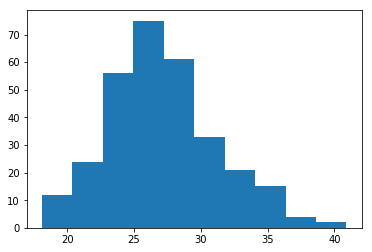
\includegraphics[width=0.95\columnwidth]{images/output_2_0.png}

\subsection{Taking all categorical features that have only 2 levels and label encoding them to get binary features}

Data preparation for data analysis is a pivotal step to take in any big data analysis. This involve manipulation of data into a form suitable for further analysis and processing. It is a process that involves many different tasks and which cannot be fully automated. Many of the data preparation activities are routine, tedious, and time consuming

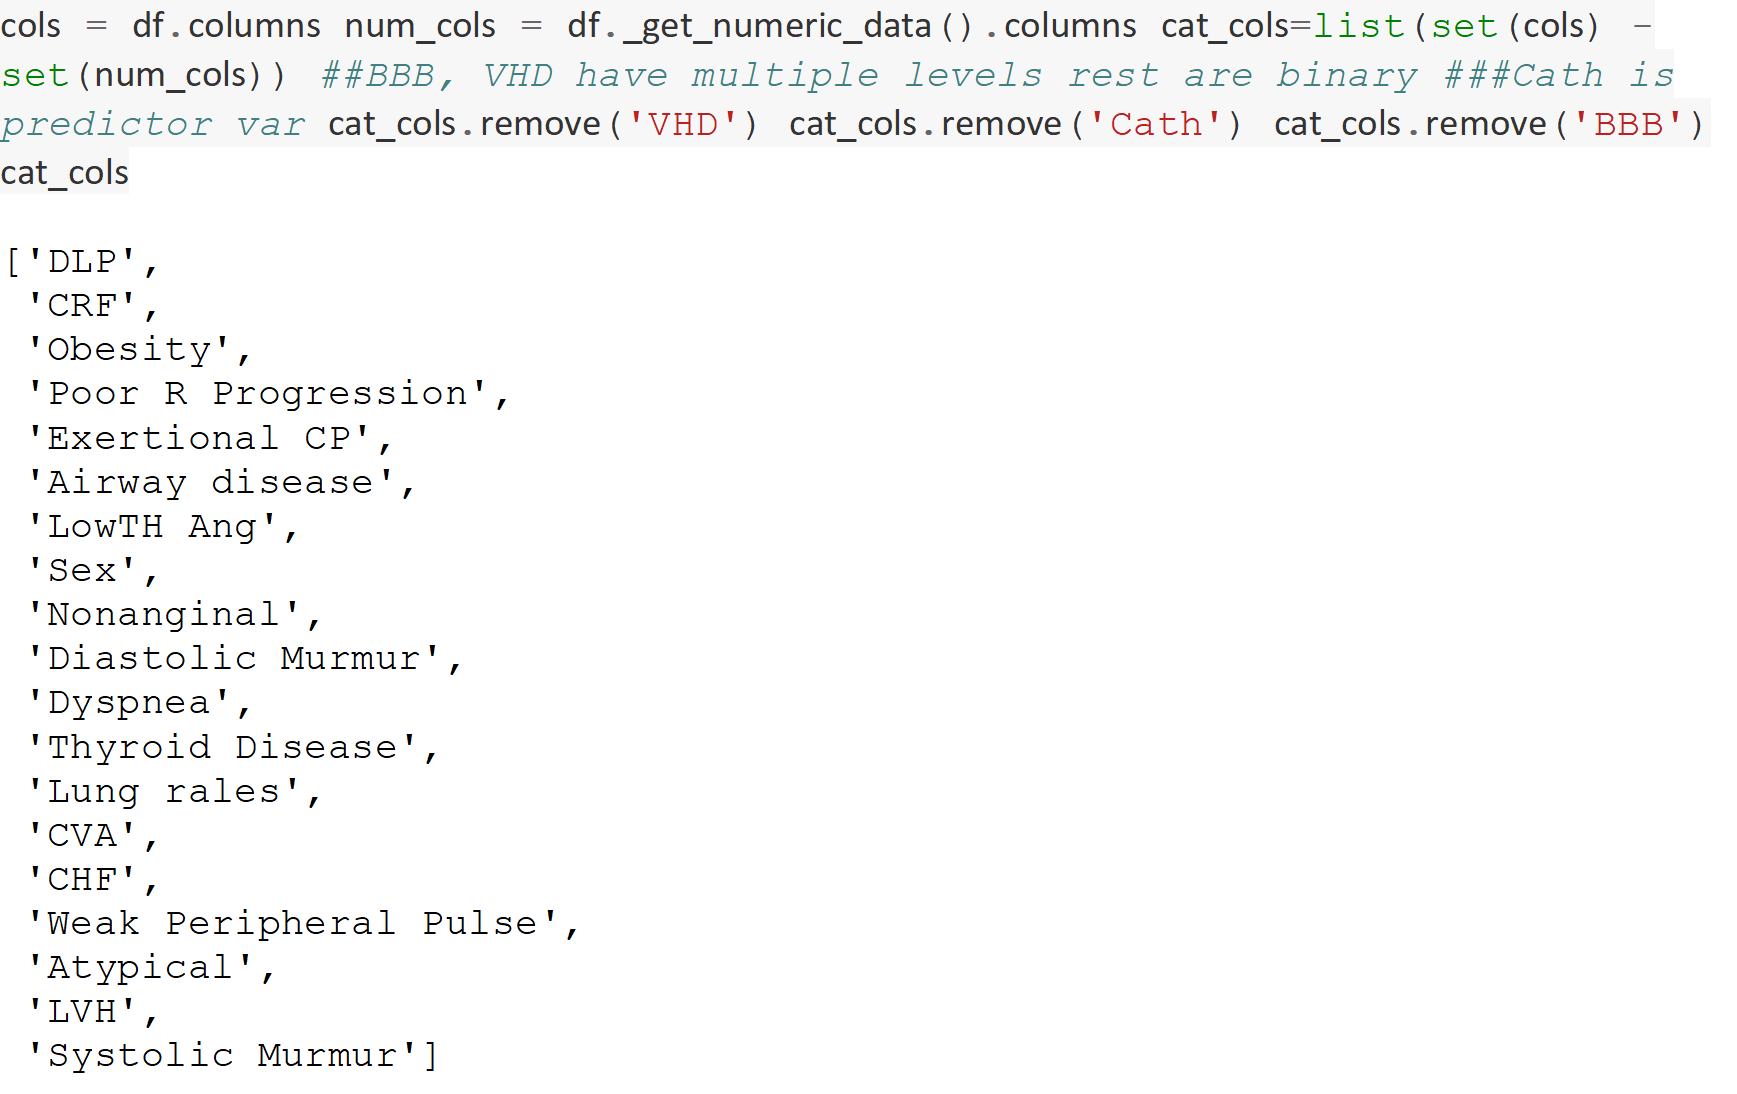
\includegraphics[width=0.95\columnwidth]{images/Untitled3.png}

\subsection{Selection of Features}

While selecting the element, the study considers the data gain measurement. Among the features, the research selects sixteen with the highest information gain and starts applying algorithms to them. Data gain shows how an element can divide several classes. For instance, is a feature separates the two classes completely; it has the highest information gain.

This layout The features with High Confidence in Predicting coronary altery disease:


['CRF',
    'Obesity',
    'Poor R Progression',
    'Exertional CP',
    'Airway disease',
    'LowTH Ang',
    'Sex',
    'Nonanginal',
    'Diastolic Murmur',
    'Dyspnea',
    'Thyroid Disease',
   'Lung rales',
    'CVA',
    'CHF',
    'Weak Peripheral Pulse',
    'Atypical',
    'LVH',
    'Systolic Murmur']
\subsection{Fitting our Encoder}

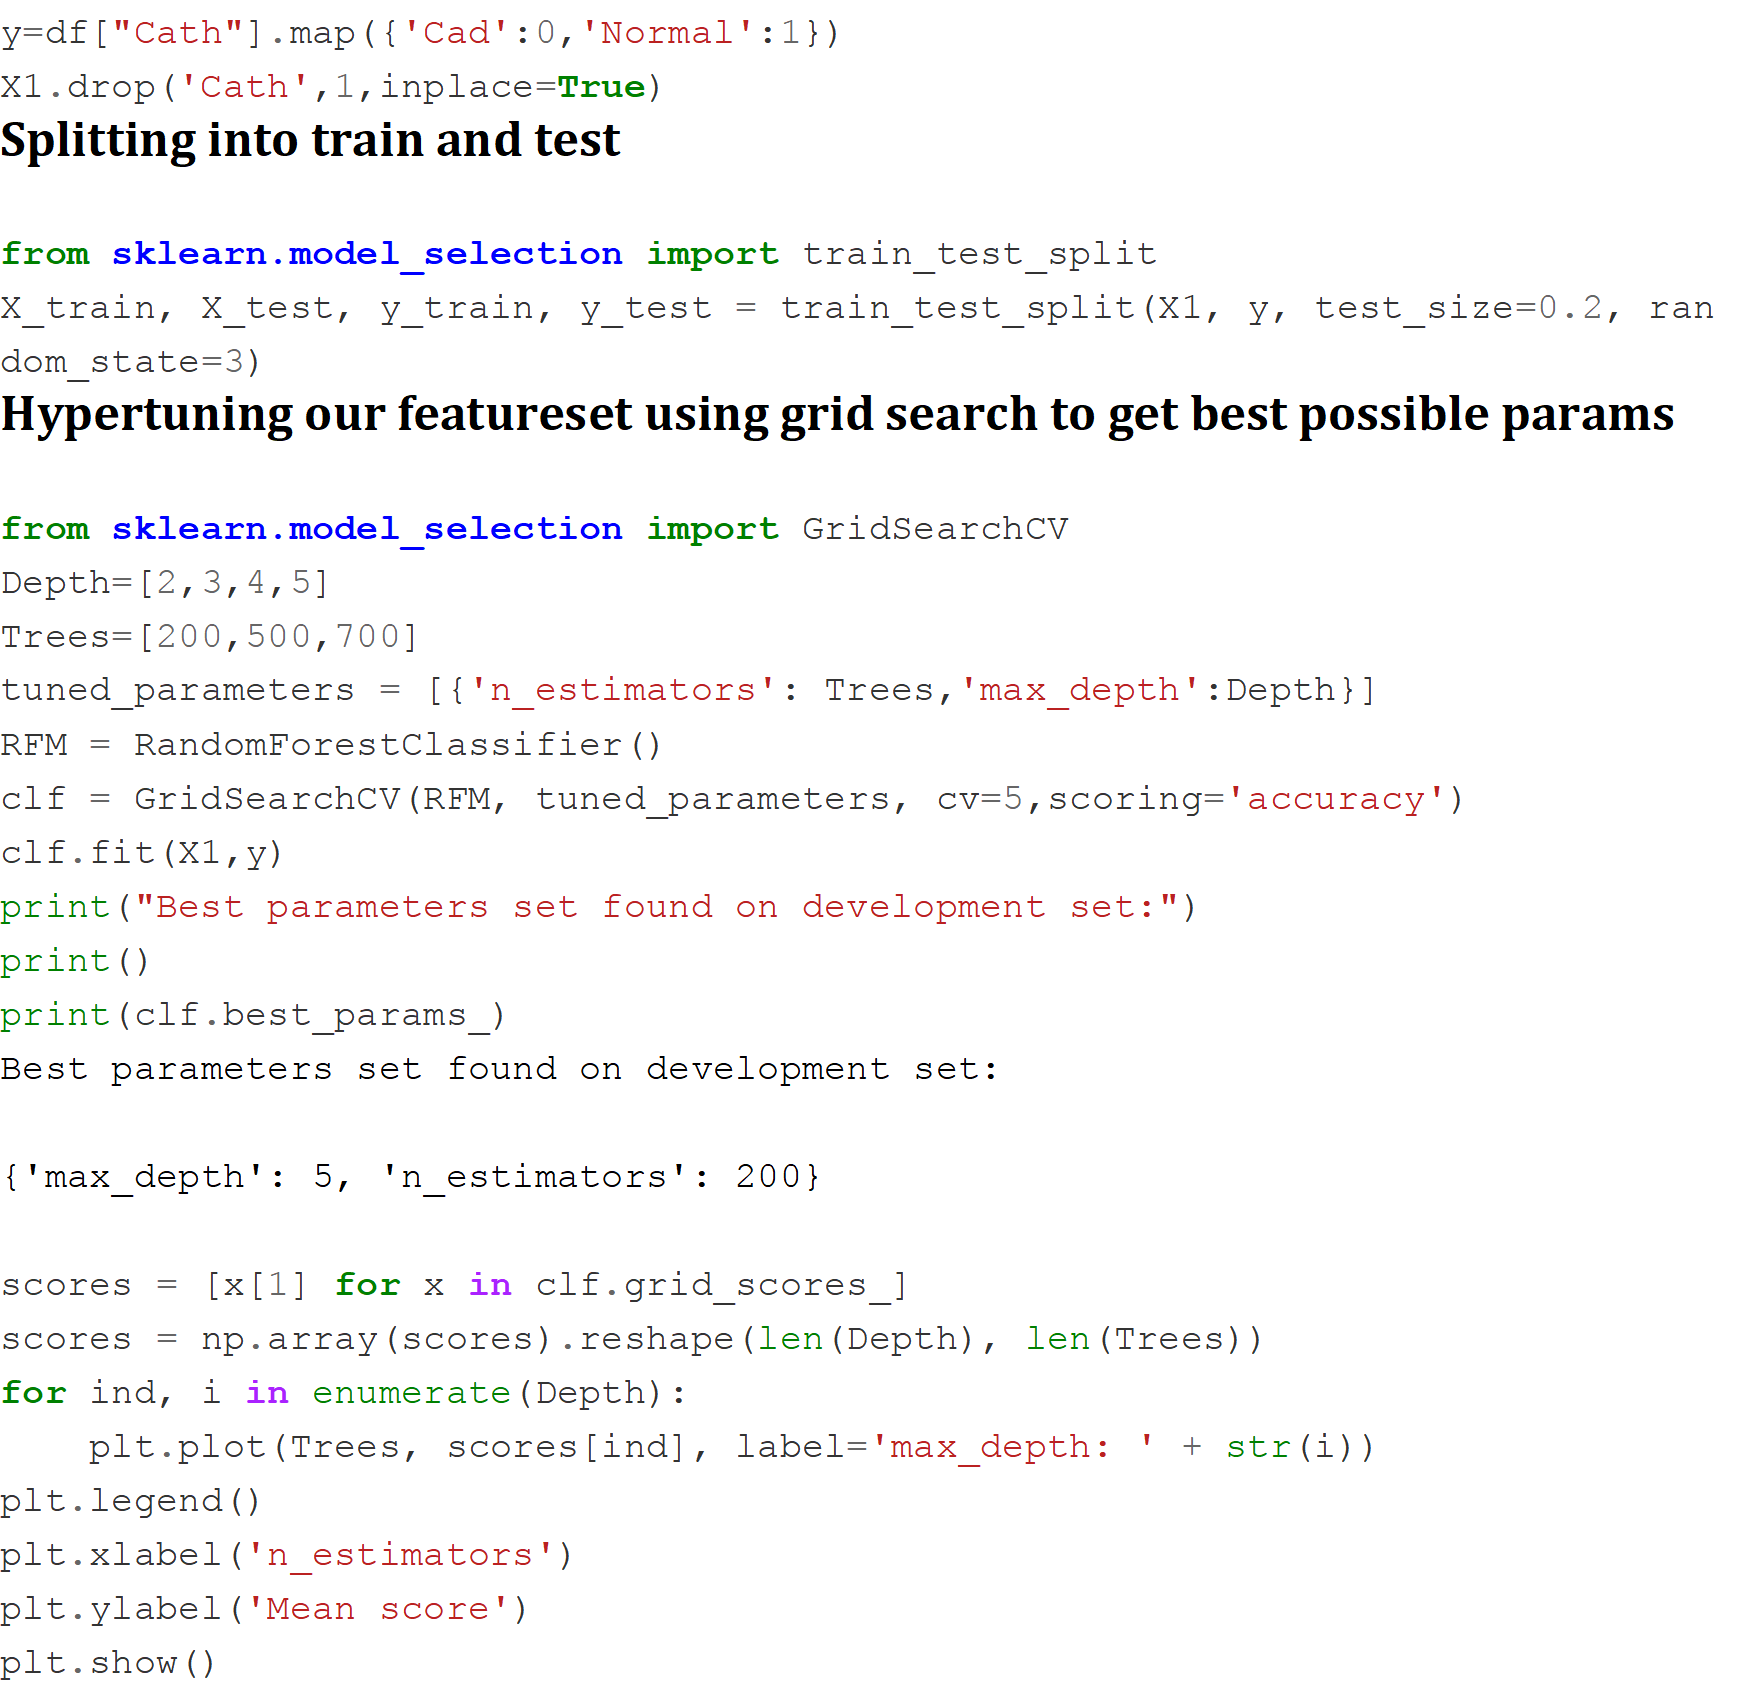
\includegraphics[width=0.95\columnwidth]{images/Untitled5.png}

\subsection{Splitting into train and test}\

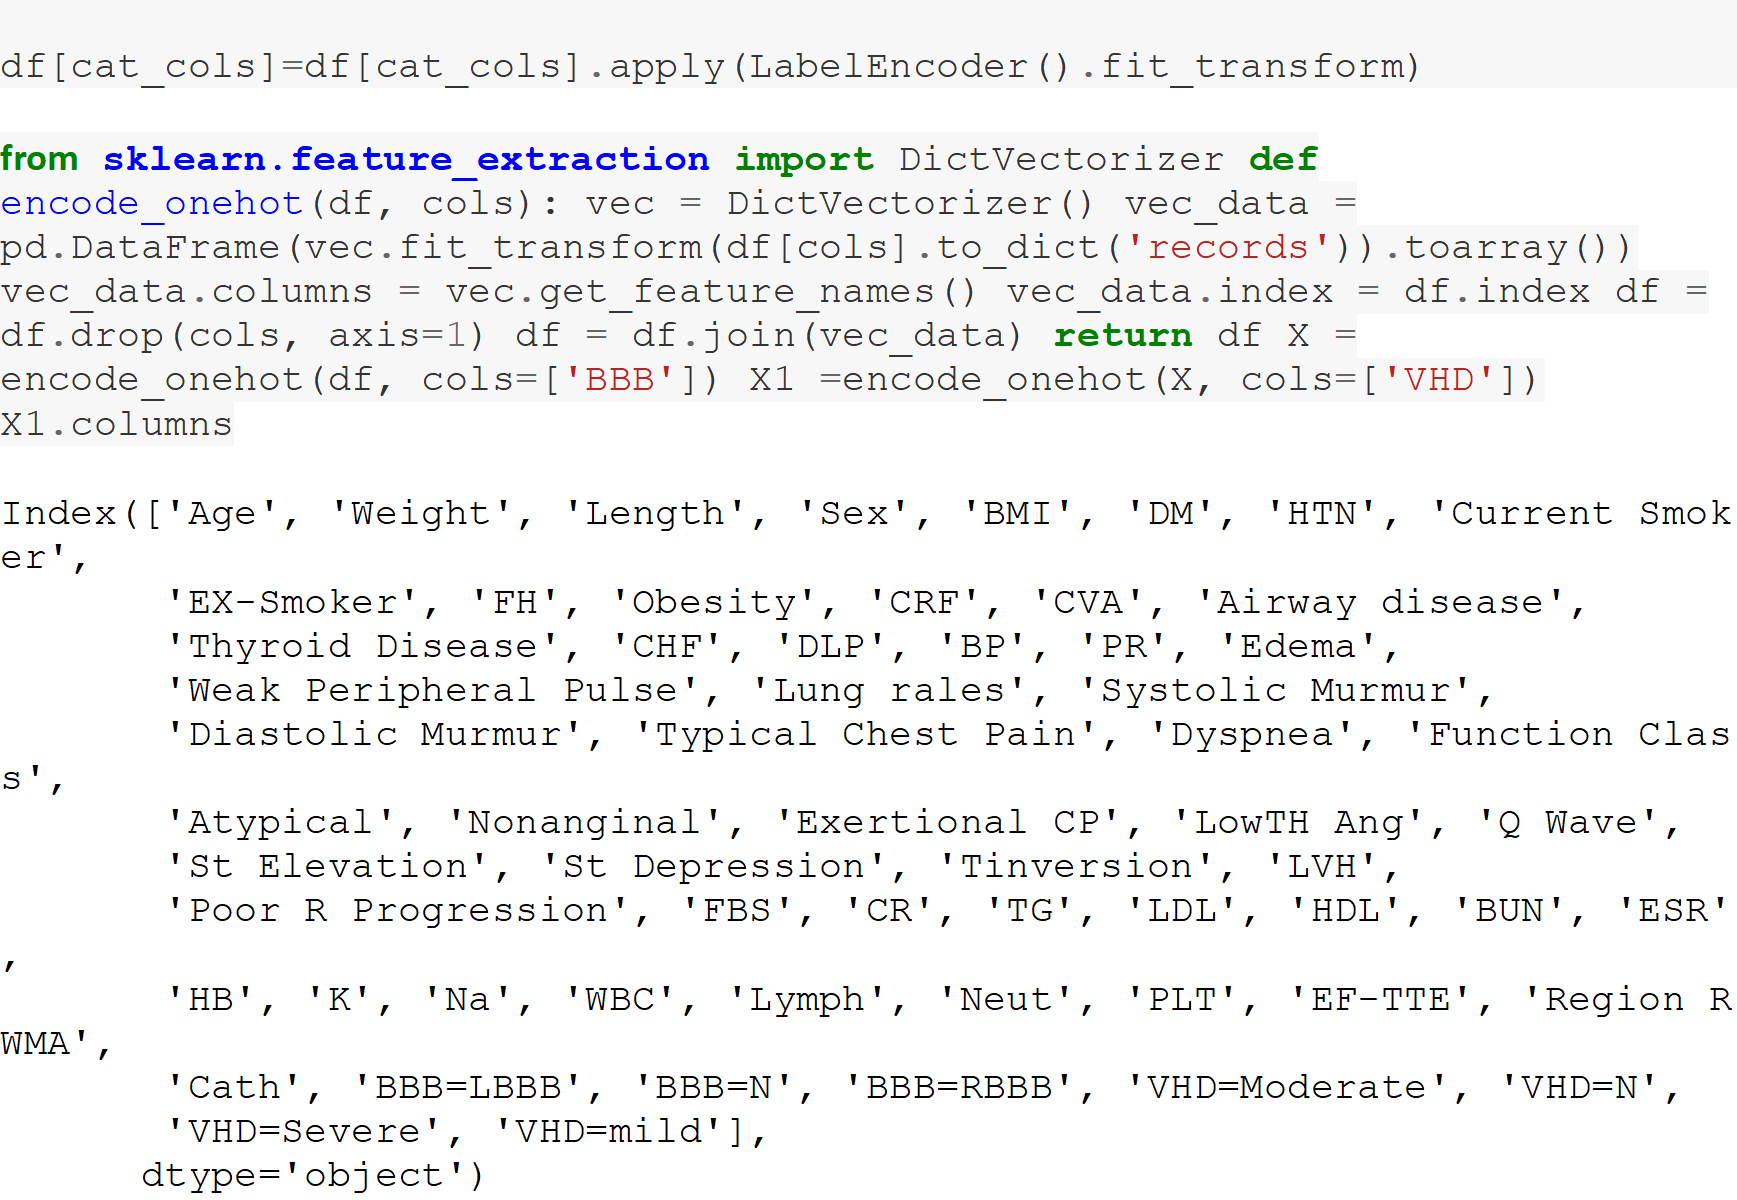
\includegraphics[width=0.95\columnwidth]{images/Untitled4.png}

Best parameters set found on development set:

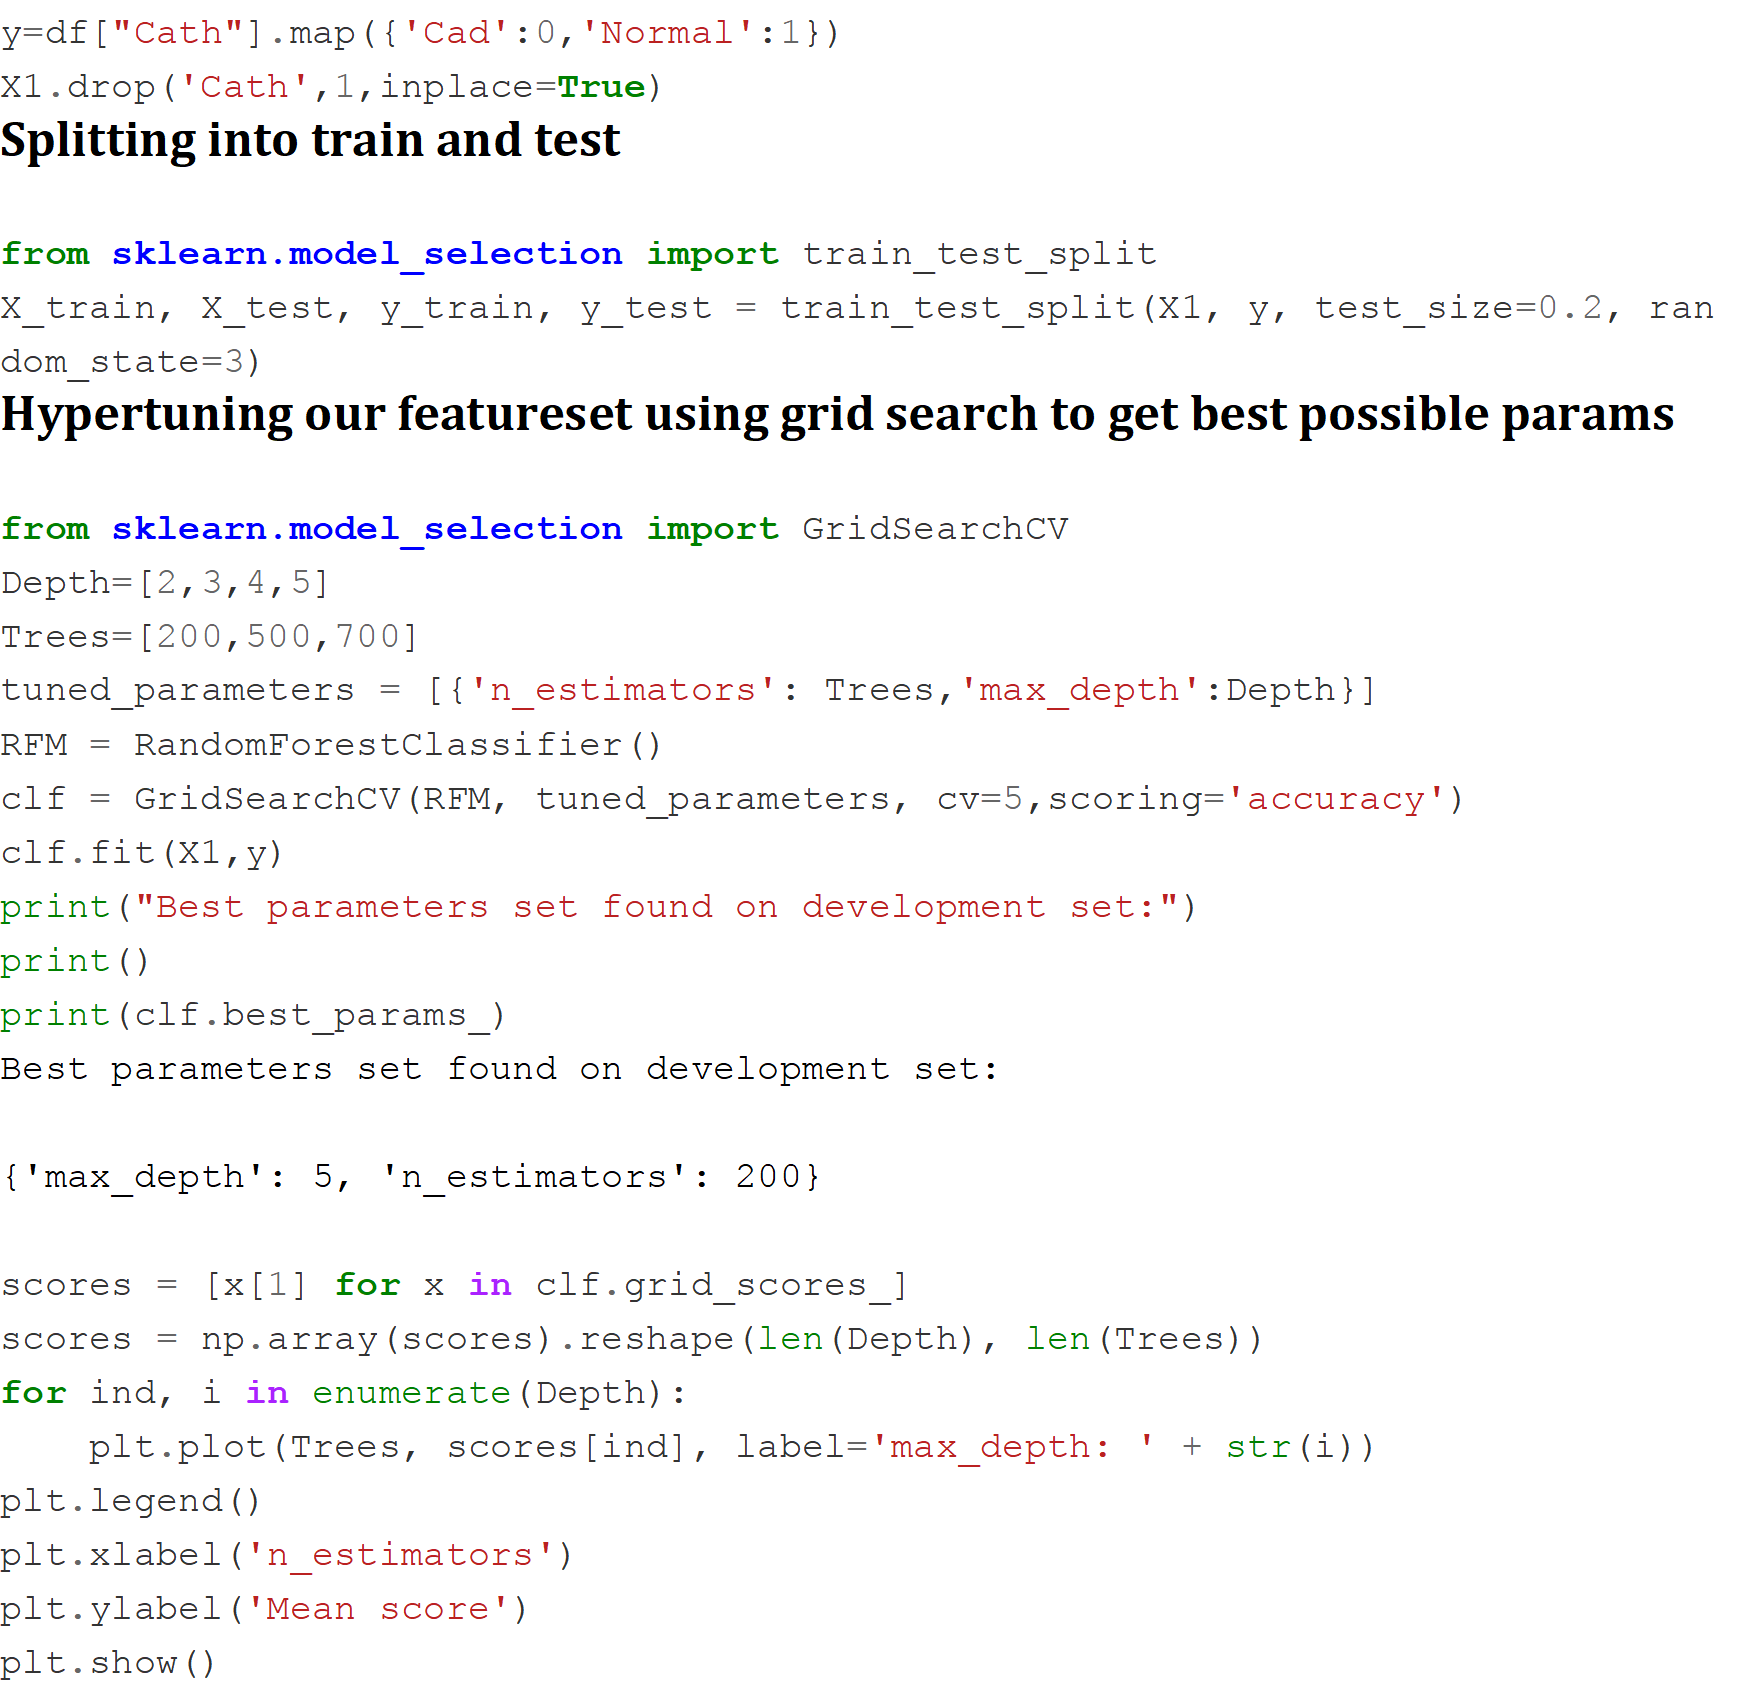
\includegraphics[width=0.95\columnwidth]{images/Untitled5.png}
`

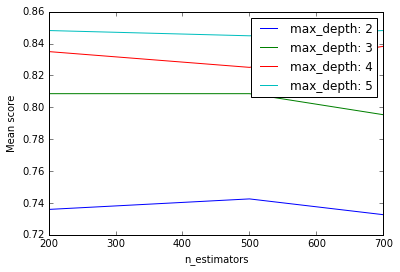
\includegraphics[width=0.95\columnwidth]{images/output_15_1.png}

This is for plotting our feature importances with their standard deviations:

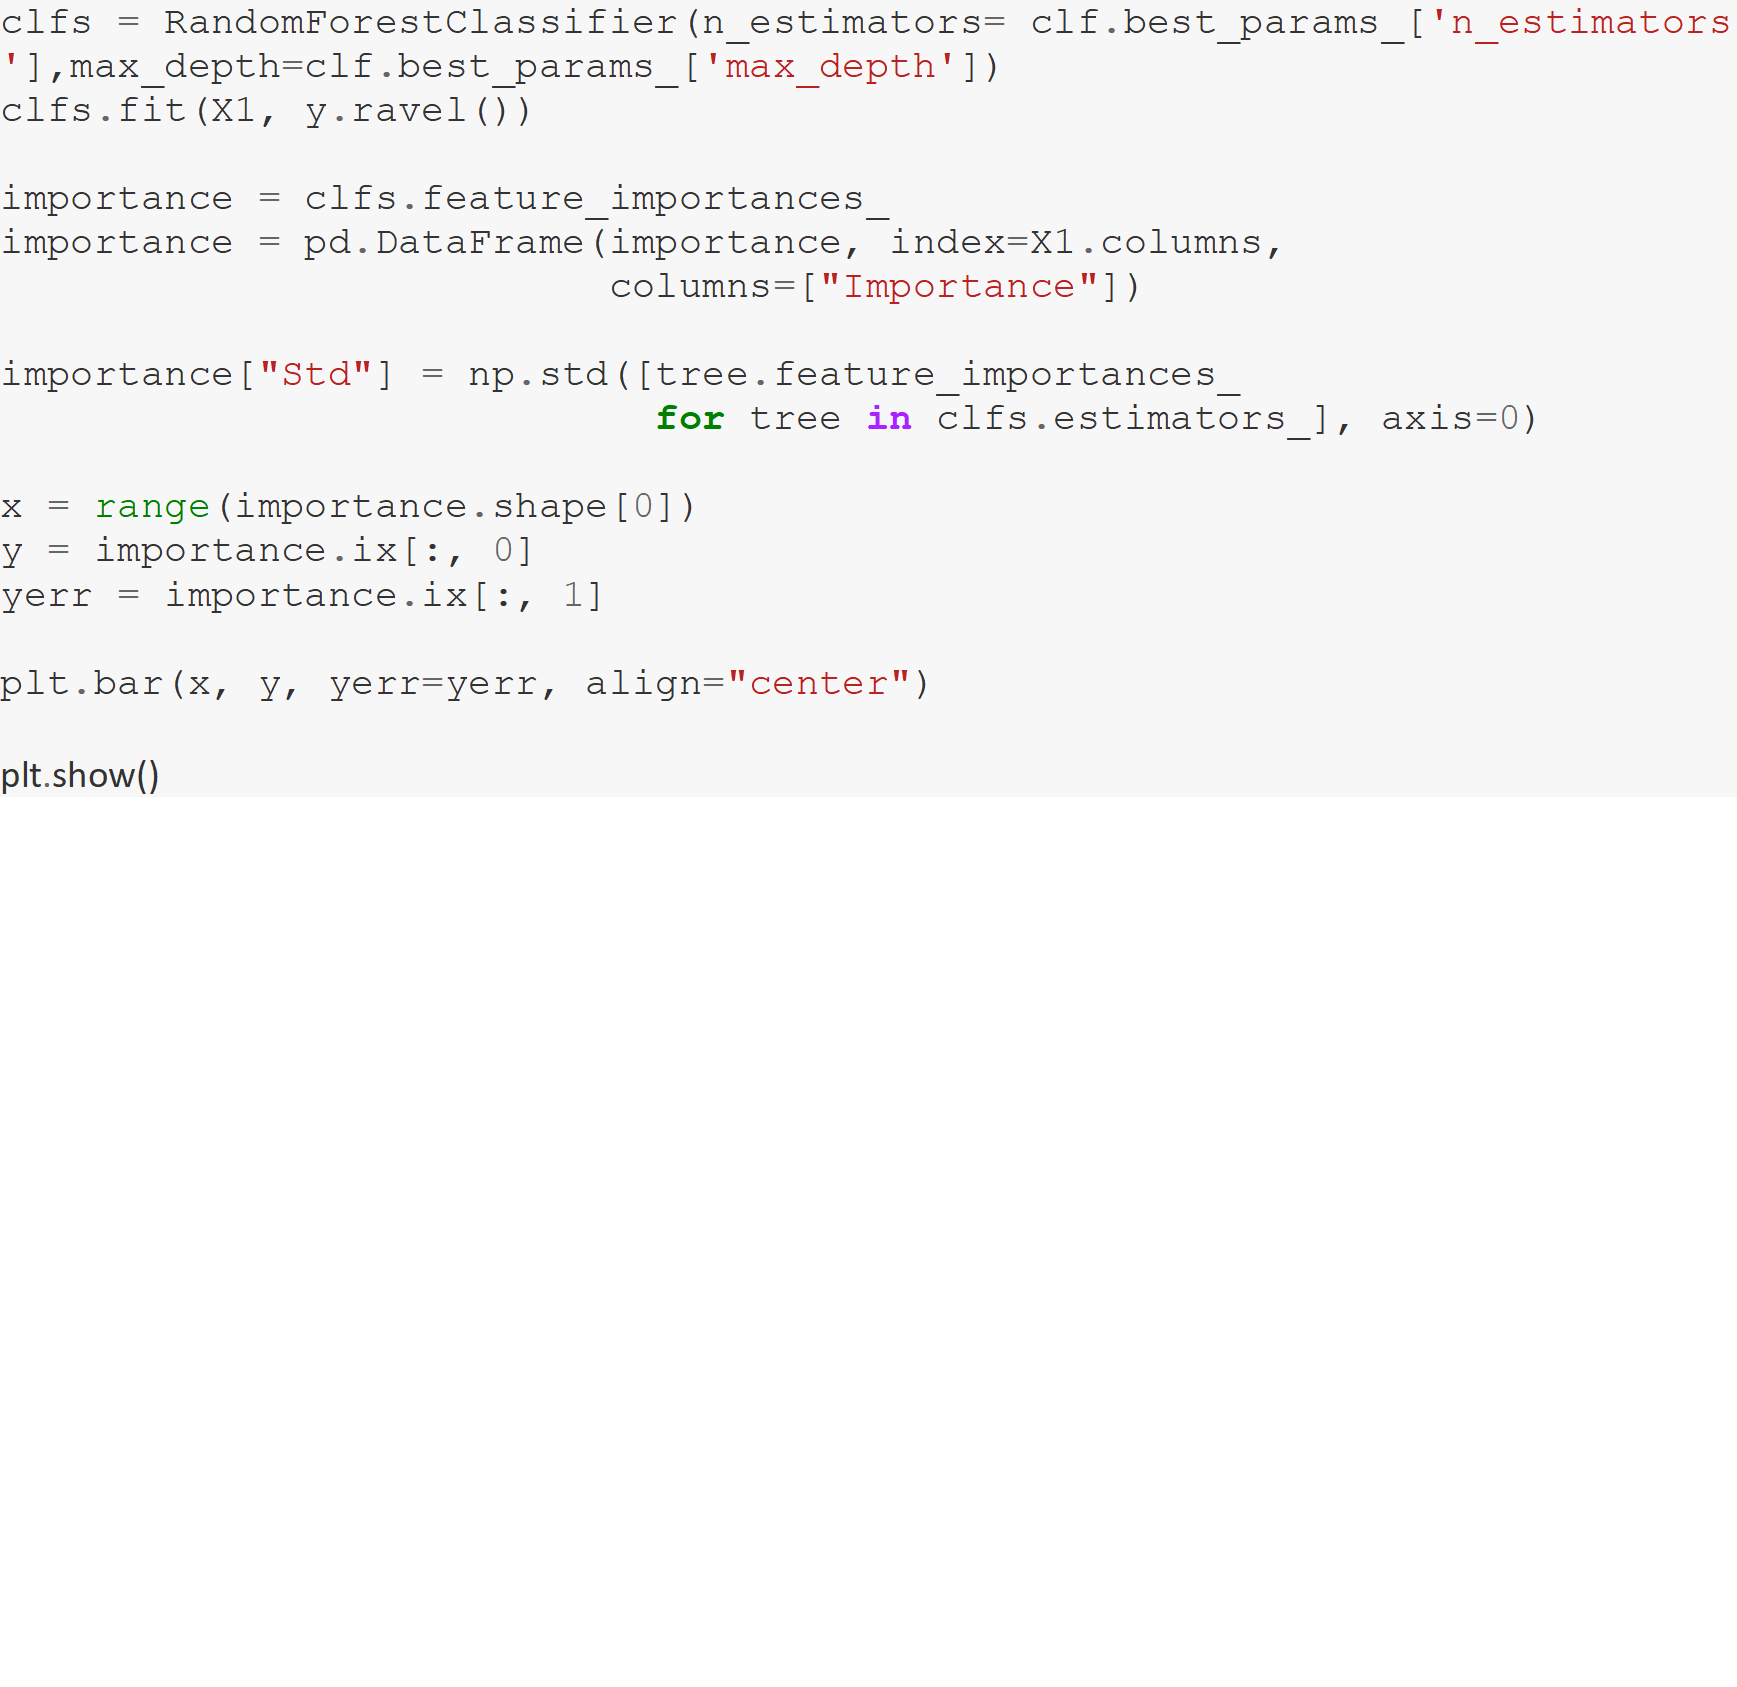
\includegraphics[width=0.95\columnwidth]{images/Untitled6.png}

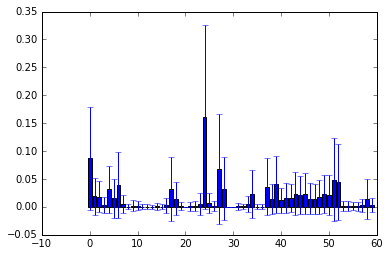
\includegraphics[width=0.95\columnwidth]{images/output_17_0.png}


\subsection{Importance}

This table show the importance of each feature in the diagnostic of CAD. Based on the analysis the age, HTN,  DM, BP, Typical chest pain, Non-Anginal  CP, T  inversion, Q  wave,  ST elevation, PR, and ST depression are the features with the highest impact on CAD.

Variable significance is figured restrictively to a given acknowledgment notwithstanding for reproduced datasets. This decision which is criticizable if the goal is to achieve a decent estimation of a basic steady, is predictable with remaining as near as conceivable to the exploratory circumstance managing a given dataset\cite{GENUER20102225}.

\begin{table}[]
\centering
\caption{Feature Importance Table}
\label{my-label}
\begin{tabular}{lll}
Importance            & Std      &          \\
Age                   & 0.086779 & 0.092552 \\
Weight                & 0.018672 & 0.032956 \\
Length                & 0.018183 & 0.027928 \\
Sex                   & 0.003414 & 0.013603 \\
BMI                   & 0.031609 & 0.042215 \\
DM                    & 0.015427 & 0.034442 \\
HTN                   & 0.038735 & 0.059296 \\
Current Smoker        & 0.005287 & 0.015965 \\
EX-Smoker             & 0.000587 & 0.004463 \\
FH                    & 0.002472 & 0.010216 \\
Obesity               & 0.002333 & 0.008439 \\
CRF                   & 0.000534 & 0.004805 \\
CVA                   & 0.000469 & 0.004108 \\
Airway disease        & 0.000474 & 0.003385 \\
Thyroid Disease       & 0.001086 & 0.006045 \\
DLP                   & 0.000407 & 0.004046 \\
BP                    & 0.003296 & 0.013382 \\
PR                    & 0.031988 & 0.056958 \\
Edema                 & 0.014277 & 0.029568 \\
Weak Peripheral Pulse & 0.001758 & 0.007496 \\
Lung rales            & 0        & 0        \\
Systolic Murmur       & 0.001332 & 0.007931 \\
Diastolic Murmur      & 0.001853 & 0.008916 \\
Typical Chest Pain    & 0.00495  & 0.020264 \\
Dyspnea               & 0.161378 & 0.165277 \\
Function Class        & 0.006237 & 0.01781  \\
Atypical              & 0.001798 & 0.008412 \\
Nonanginal            & 0.067681 & 0.098911 \\
Exertional CP         & 0.032299 & 0.056285 \\
LowTH Ang             & 0        & 0        \\
Q Wave                & 0        & 0        \\
St Elevation          & 0.000976 & 0.005923 \\
St Depression         & 0.005336 & 0.014798
\end{tabular}
\end{table}

\subsection{Model Accuracy}  

Finally by checking of our model's accuracy on test set 0.885245901639.

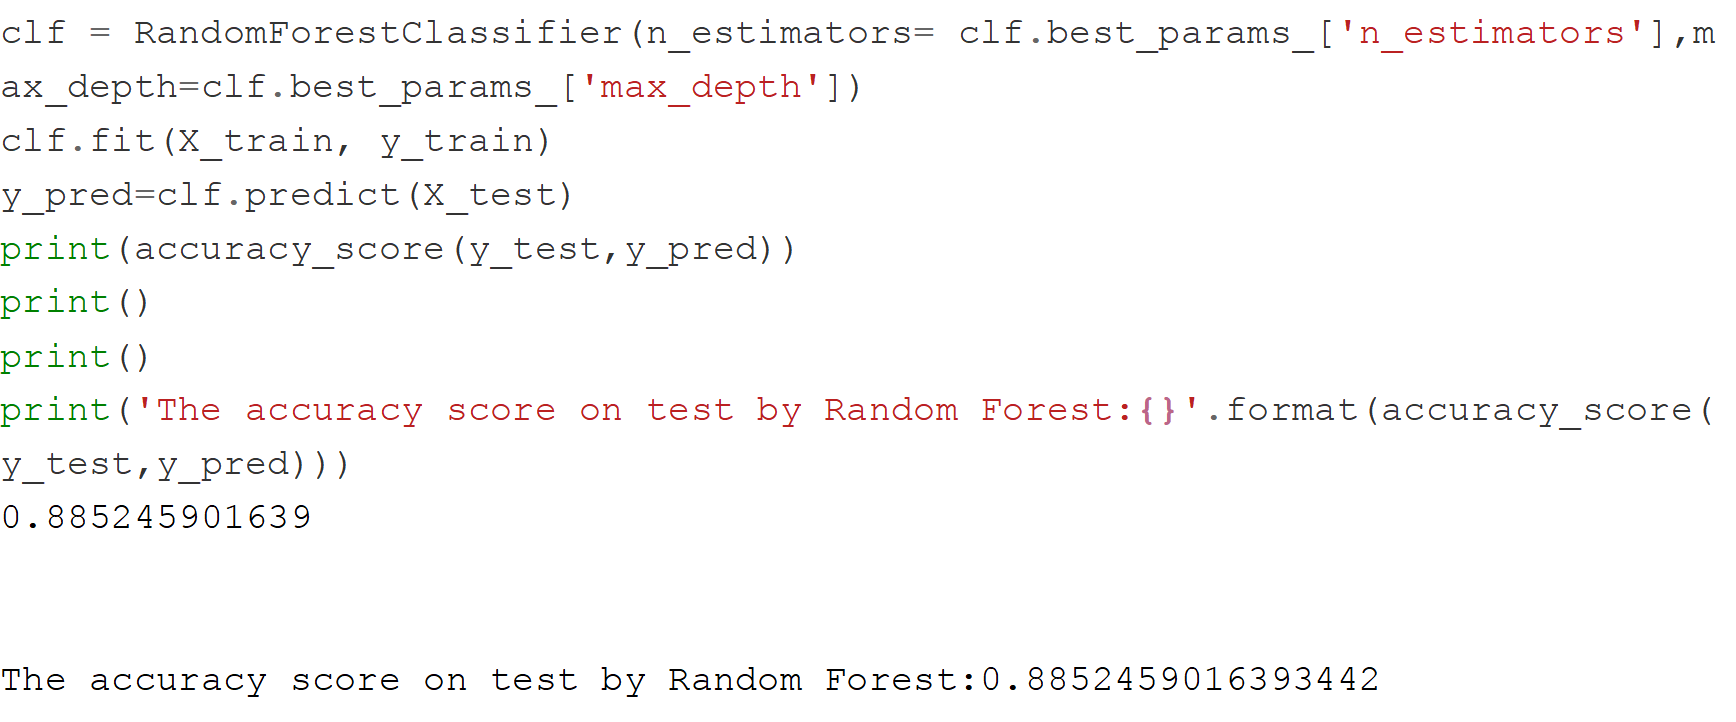
\includegraphics[width=0.95\columnwidth]{images/Untitled7.png}

The study shows that the ensemble technique it proposes has a higher accuracy rate than the SMO and Naïve methods, while the two techniques have almost the same accuracy's. Furthermore, the HTN, typical chest pain, ST elevation, BP, PR features, T inversion, and DM have an impact on CAD. The research also show that the association rule mining method results in laws with high confidences. The research also shows that the ensemble method is the best among the three because it combines both of the as its features. Unfortunately, the technique comprising both Naïve method and SMO technique makes it easier to fail; this is in case one of them has a problem, the entire system fails.

\subsection{Conclusion}

A period of open data in social insurance is currently under way. We have effectively encountered a time of advance in digitizing therapeutic records, as pharmaceutical organizations and different associations total a long time of innovative work information in electronic databases. The national government and other open partners have additionally quickened the push toward straightforwardness by making many years of put away information usable, accessible, and significant by the medicinal services segment in general. Together, these increments in information liquidity have conveyed the business to the tipping point.

\subsection{Acknowlement}

  I would like to thank Dr. Gregor von Laszewski for his
  support and suggestions to write this paper.




    
    
    


    % Add a bibliography block to the postdoc
    \bibliographystyle{acm}
    \bibliography{report}
    
    \end{document}
